\documentclass[a4paper,12pt]{extarticle}
\usepackage[utf8x]{inputenc}
\usepackage[T1,T2A]{fontenc}
\usepackage[russian]{babel}
\usepackage{hyperref}
\usepackage{indentfirst}
\usepackage{listings}
\usepackage{color}
\usepackage{here}
\usepackage{array}
\usepackage{multirow}
\usepackage{graphicx}

\usepackage{amsmath}

\usepackage{caption}
\renewcommand{\lstlistingname}{Программа} % заголовок листингов кода

\bibliographystyle{ugost2008ls}

\usepackage{listings}
\lstset{ %
extendedchars=\true,
keepspaces=true,
language=C,						% choose the language of the code
basicstyle=\footnotesize,		% the size of the fonts that are used for the code
numbers=left,					% where to put the line-numbers
numberstyle=\footnotesize,		% the size of the fonts that are used for the line-numbers
stepnumber=1,					% the step between two line-numbers. If it is 1 each line will be numbered
numbersep=5pt,					% how far the line-numbers are from the code
backgroundcolor=\color{white},	% choose the background color. You must add \usepackage{color}
showspaces=false				% show spaces adding particular underscores
showstringspaces=false,			% underline spaces within strings
showtabs=false,					% show tabs within strings adding particular underscores
frame=single,           		% adds a frame around the code
tabsize=2,						% sets default tabsize to 2 spaces
captionpos=t,					% sets the caption-position to top
breaklines=true,				% sets automatic line breaking
breakatwhitespace=false,		% sets if automatic breaks should only happen at whitespace
escapeinside={\%*}{*)},			% if you want to add a comment within your code
postbreak=\raisebox{0ex}[0ex][0ex]{\ensuremath{\color{red}\hookrightarrow\space}},
texcl=true,
inputpath=listings,                     % директория с листингами
}

\usepackage[left=2cm,right=2cm,
top=2cm,bottom=2cm,bindingoffset=0cm]{geometry}

%% Нумерация картинок по секциям
\usepackage{chngcntr}
\counterwithin{figure}{section}
\counterwithin{table}{section}

%%Точки нумерации заголовков
\usepackage{titlesec}
\titlelabel{\thetitle.\quad}
\usepackage[dotinlabels]{titletoc}

%% Оформления подписи рисунка
\addto\captionsrussian{\renewcommand{\figurename}{Рисунок}}
\captionsetup[figure]{labelsep = period}

%% Подпись таблицы
\DeclareCaptionFormat{hfillstart}{\hfill#1#2#3\par}
\captionsetup[table]{format=hfillstart,labelsep=newline,justification=centering,skip=-10pt,textfont=bf}

%% Путь к каталогу с рисунками
\graphicspath{{fig/}}


\begin{document}	% начало документа

% Титульная страница
\begin{titlepage}	% начало титульной страницы

	\begin{center}		% выравнивание по центру

		\large Санкт-Петербургский Политехнический Университет Петра Великого\\
		\large Институт компьютерных наук и технологий \\
		\large Кафедра компьютерных систем и программных технологий\\[6cm]
		% название института, затем отступ 6см
		
		\huge Телекоммуникационные технологии\\[0.5cm] % название работы, затем отступ 0,5см
		\large Отчет по лабораторной работе №4\\[0.1cm]
		\large Аналоговая модуляция\\[5cm]

	\end{center}


	\begin{flushright} % выравнивание по правому краю
		\begin{minipage}{0.25\textwidth} % врезка в половину ширины текста
			\begin{flushleft} % выровнять её содержимое по левому краю

				\large\textbf{Работу выполнил:}\\
				\large Соболь В.О.\\
				\large {Группа:} 33501/4\\
				
				\large \textbf{Преподаватель:}\\
				\large Богач Н.В.

			\end{flushleft}
		\end{minipage}
	\end{flushright}
	
	\vfill % заполнить всё доступное ниже пространство

	\begin{center}
	\large Санкт-Петербург\\
	\large \the\year % вывести дату
	\end{center} % закончить выравнивание по центру

\thispagestyle{empty} % не нумеровать страницу
\end{titlepage} % конец титульной страницы

\vfill % заполнить всё доступное ниже пространство

% Содержание
% Содержание
\renewcommand\contentsname{\centerline{Содержание}}
\tableofcontents
\newpage




\section{Цель работы}
Изучить воздействие фильтра нижних частот на тестовый сигнал с шумом.

\section{Постановка задачи}
Сгенерировать тестовый гармонический сигнал с шумом, синтезировать ФНЧ, отфильтровать сигнал с шумом. Посмотреть, как ФНЧ влияет на спектр сигнала.

\section{Теоретическая информация}
\subsection{Генерация гармонического сигнала с шумом}
Для генерации гармонического сигнала можно воспользоваться формулой $signal = A*cos(2*\pi * f*t + \varphi)$,
 где $ A $ --- амплитуда сигнала, $f$ --- частота, $t$ --- вектор отсчетов времени, $\varphi$ --- смещение по фазе.

Для добавления шума в исходный сигнал необходимо сложить его с другим сигналом, полученным по аналогичной формуле, но для другой частоты.

\subsection{Фильтр нижних частот}
Любой фильтр работает по принципу умножения сигнала в частотной области на коэффициент, зависящий от частоты.
Фильтр усиливает (или не изменяет) частоты в диапазоне и ослабляет вне его. Так, фильтр нижних частот ослабляет частоты выше заданной границы, умножая их на маленький коэффициент. АЧХ такого фильтра показана на рис.\ref{pic:ach_fnc}:
\begin{figure}[H]
	\begin{center}
		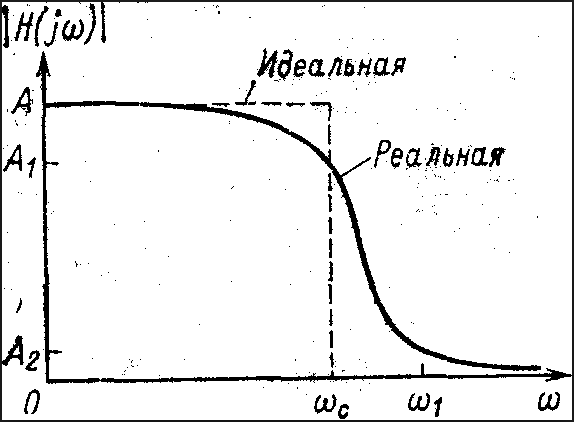
\includegraphics[scale=0.7]{ach_fnc}
		\caption{АЧХ фильтра нижних частот} 
		\label{pic:ach_fnc} % название для ссылок внутри кода
	\end{center}
\end{figure}

Фильтры делятся на БИХ (с бесконечной импульсной характеристикой) и КИХ (с конечной импульсной характеристикой).
Основным свойством БИХ фильтров является то, что их импульсная переходная характеристика имеет бесконечную длину во временной области. У КИХ фильтров гарантируется, что с какого-то момента импульсная характеристика станет равна 0.
Это делает их более устойчивыми, по сравнению с БИХ фильтрами. Самая важная особенность КИХ фильтров заключается в возможности получения точной линейной фазовой характеристики. 

Основным методом расчета коэффициентов является модифицированный алгоритм Ремеза --- (Parks-McClellan algorithm). 
Это косвенный итерационный метод для нахождения оптимальных значений с Чебышевской характеристикой фильтра.
 Особенность метода заключается в минимизации ошибки в полосе затухания и пропускания путем Чебышевской аппроксимации импульсной характеристики.
 
В работе используется КИХ фильтр с равномерно пульсирующей АЧХ (equiriple filter). 

\section{Ход работы}

Ход работы можно разделить на 2 части - генерация зашумлённого сигнала и фильтрация этого сигнала.
Код использованный при исследовании приведён в листинге~\ref{code:code}.

\subsection{Генерация гармонического сигнала с шумом}
Для начала получим обычный гармонический сигнал с частотой 30 Гц. Сгенерированный сигнал представлен на рисунке \ref{pic:signal1}:
\begin{figure}[H]
	\begin{center}
		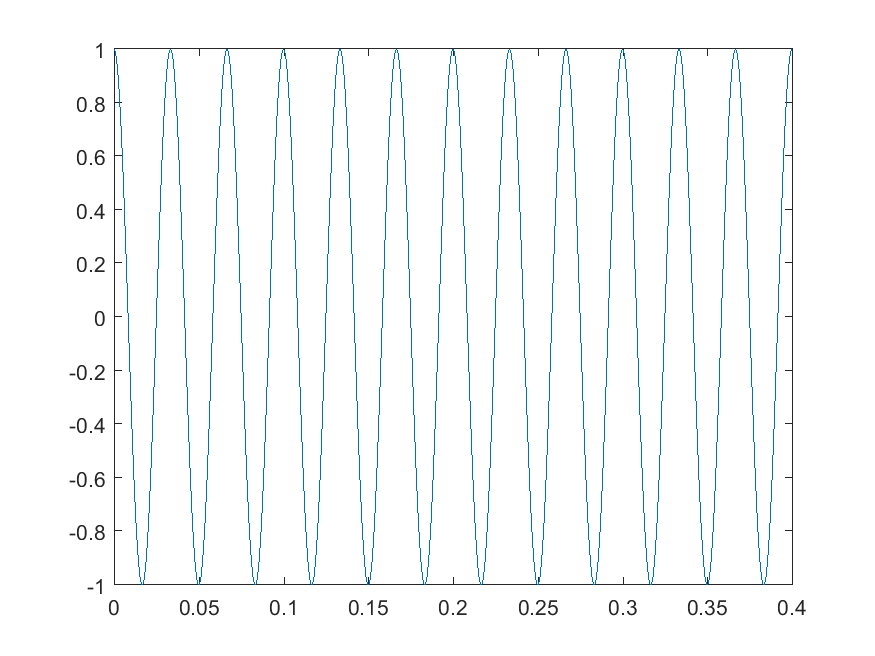
\includegraphics[scale=0.7]{signal1}
		\caption{Гармонический сигнал} 
		\label{pic:signal1} % название для ссылок внутри кода
	\end{center}
\end{figure}

Затем сгенерируем еще один сигнал с более высокой частотой, и прибавим его к имеющемуся. Результат добавления шума в сигнал показан на рисунке \ref{pic:signal2}:
\begin{figure}[H]
	\begin{center}
		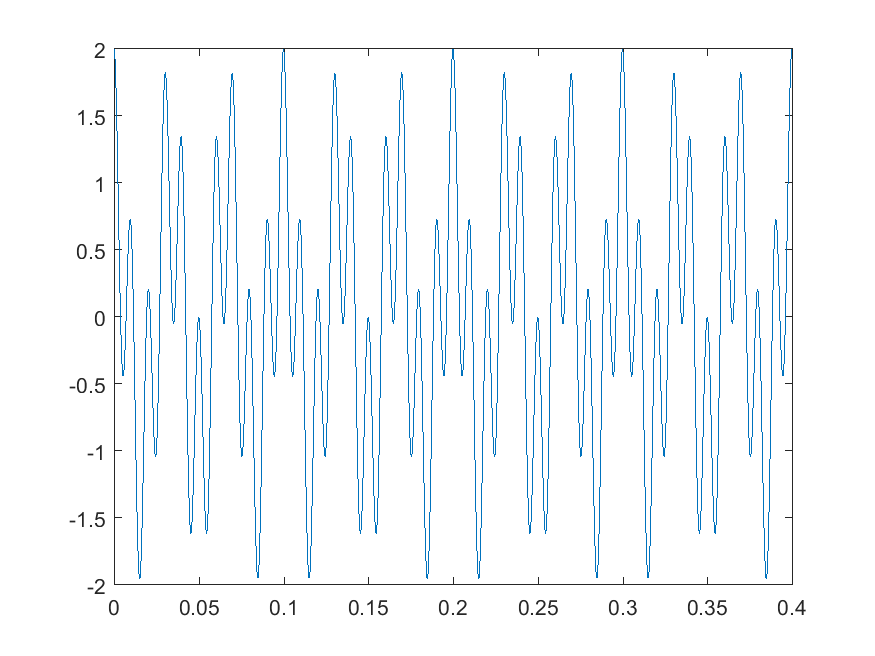
\includegraphics[scale=0.7]{signal2}
		\caption{Гармонический сигнал с шумом} 
		\label{pic:signal2} % название для ссылок внутри кода
	\end{center}
\end{figure}

Далее получим спектр сигнала с помощью преобразования Фурье. Спектр гармонического сигнала с шумом приведен на рисунке \ref{pic:signal2_fft}:
\begin{figure}[H]
	\begin{center}
		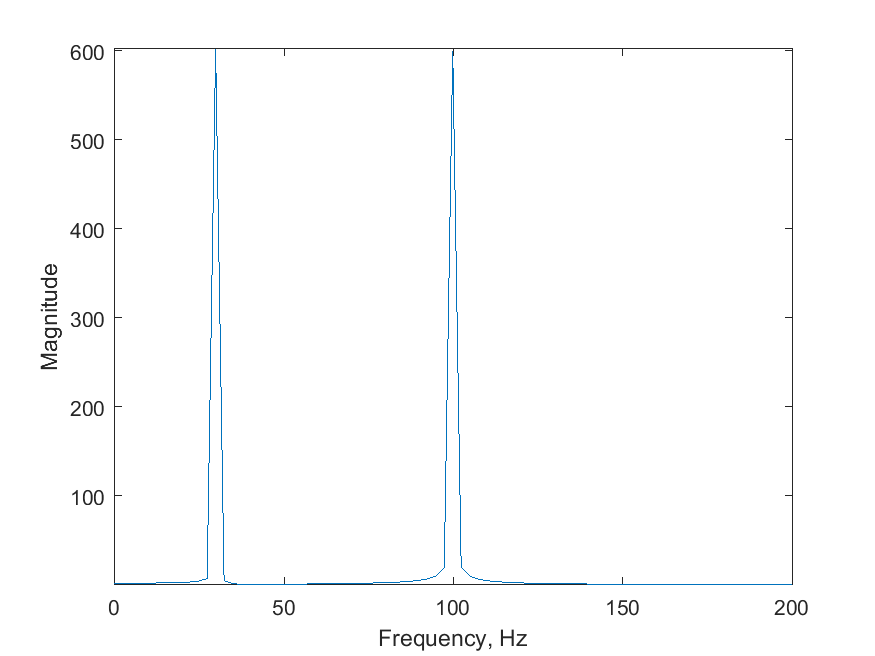
\includegraphics[scale=0.7]{signal2_fft}
		\caption{Спектр зашумленной гармоники} 
		\label{pic:signal2_fft} % название для ссылок внутри кода
	\end{center}
\end{figure}
Видно, что в сигнале присутствуют 2 гармоники разной частоты.

\subsection{Фильтрация сигнала}

Для фильтрации будем использовать КИХ фильтр низких частот с равномерно пульсирующей АЧХ. 
Коэффициенты фильтра получены с помощью функции Matlab (листинг~\ref{code:code}, строка 21)

Отфильтрованный полученным фильтром сигнал можно увидеть на рисунке \ref{pic:filter_signal}:
\begin{figure}[H]
	\begin{center}
		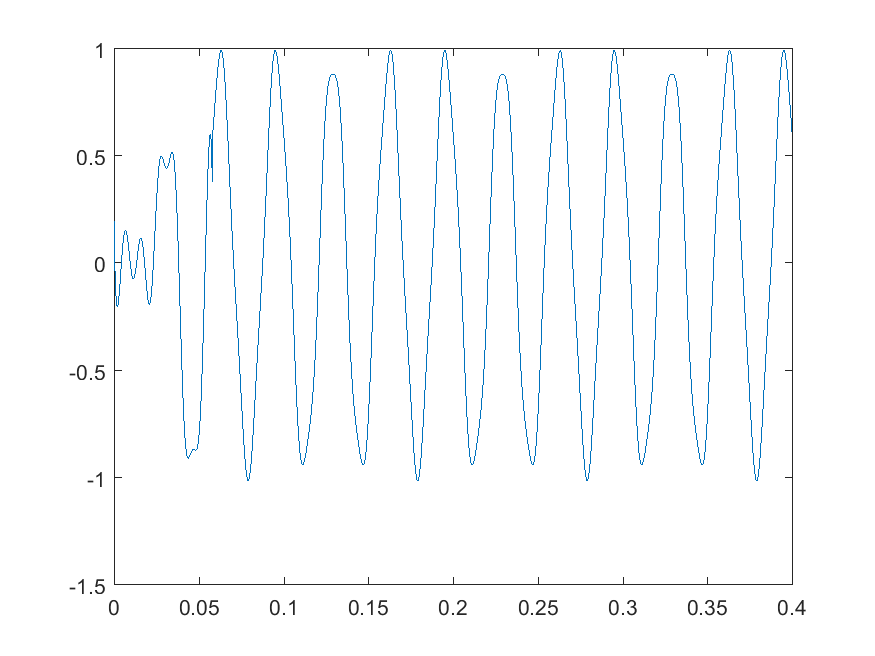
\includegraphics[scale=0.7]{filter_signal}
		\caption{Сигнал после прохождения фильтра} 
		\label{pic:filter_signal} % название для ссылок внутри кода
	\end{center}
\end{figure}
Максимальная амплитуда немного уменьшена из-за коэффициента ослабления фильтра, и сигнал устанавливается с небольшой задержкой.

Спектр данного сигнала, полученный с помощью преобразования Фурье, приведен на рисунке \ref{pic:filter_signal_fft}:
\begin{figure}[H]
	\begin{center}
		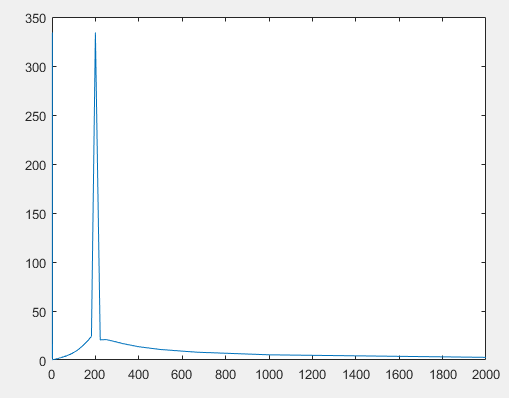
\includegraphics[scale=0.7]{filter_signal_fft}
		\caption{Спектр отфильтрованного сигнала} 
		\label{pic:filter_signal_fft} % название для ссылок внутри кода
	\end{center}
\end{figure}
На рисунке видна одна гармоника, т.е. фильтр верно отсек гармонику шума, внесенного нами в сигнал.

\section{Выводы}

Нами исследовано прохождение сигнала через линейную цепь фильтра нижних частот.
Фильтрация зашумлённого сигнала --- это свёртка с окном чистой АЧХ.
Идеальное окно имеет вид прямоугольника, но получить его невозможно. 
На практике используется не идеальная аппроксимация, с неполным подавлением 
шума на частотах, близких к частоте среза. 
Это объясняется тем, что аппроксимация имеет неидеальный наклон кривой после частоты среза.

\section{Листинг}
\lstinputlisting[
	label=code:code,
	caption={Код для исследования фильтра},
]{Code.m}
\parindent=1cm
\end{document}
